\chapter{提案}
提案手法について簡単に書く
OS仮想化基盤を用いたSBCマルチディスプレイシステムのフレーム処理並列化

\section{OS仮想化基盤とコンテナ技術}
OS仮想化基盤には,代表的なものとしてDockerが挙げられる.


\section{MDのコンテナ化}
以下,コンテナ技術を用いたSBCマルチディスプレイシステムの実装について書く

\section{コンテナを通したディスプレイの制御}
コンテナ内からディスプレイを制御する方法について書く
フレームバッファを利用したディスプレイ表示のメカニズムについて図を使って解説できると良い


\section{ヘッドノードでのフレーム処理の改良}
ヘッドノード内でのコンテナを用いたフレーム処理の並列化について書く
メインコンテナ,圧縮コンテナの実装や動作などについて図やフローチャートを用いて解説する

\subsection*{フレーム処理のコンテナ並列化}
\subsection*{コンテナ間でのフレーム受け渡し処理}
\begin{figure}[H]
    \hspace*{\fill}
    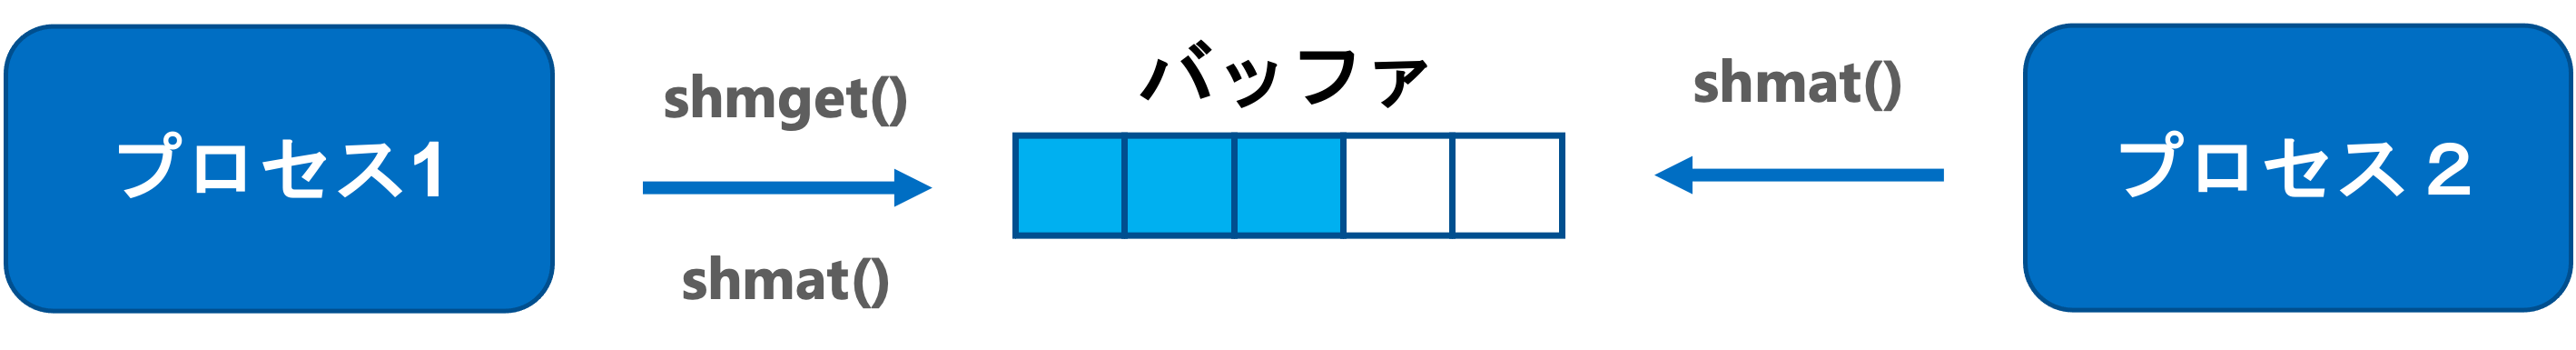
\includegraphics[width=\linewidth]{./fig/shared_memory.eps}
    \hspace*{\fill}
    \caption{共有メモリの使用例}
   \end{figure}

\begin{figure}[H]
    \hspace*{\fill}
    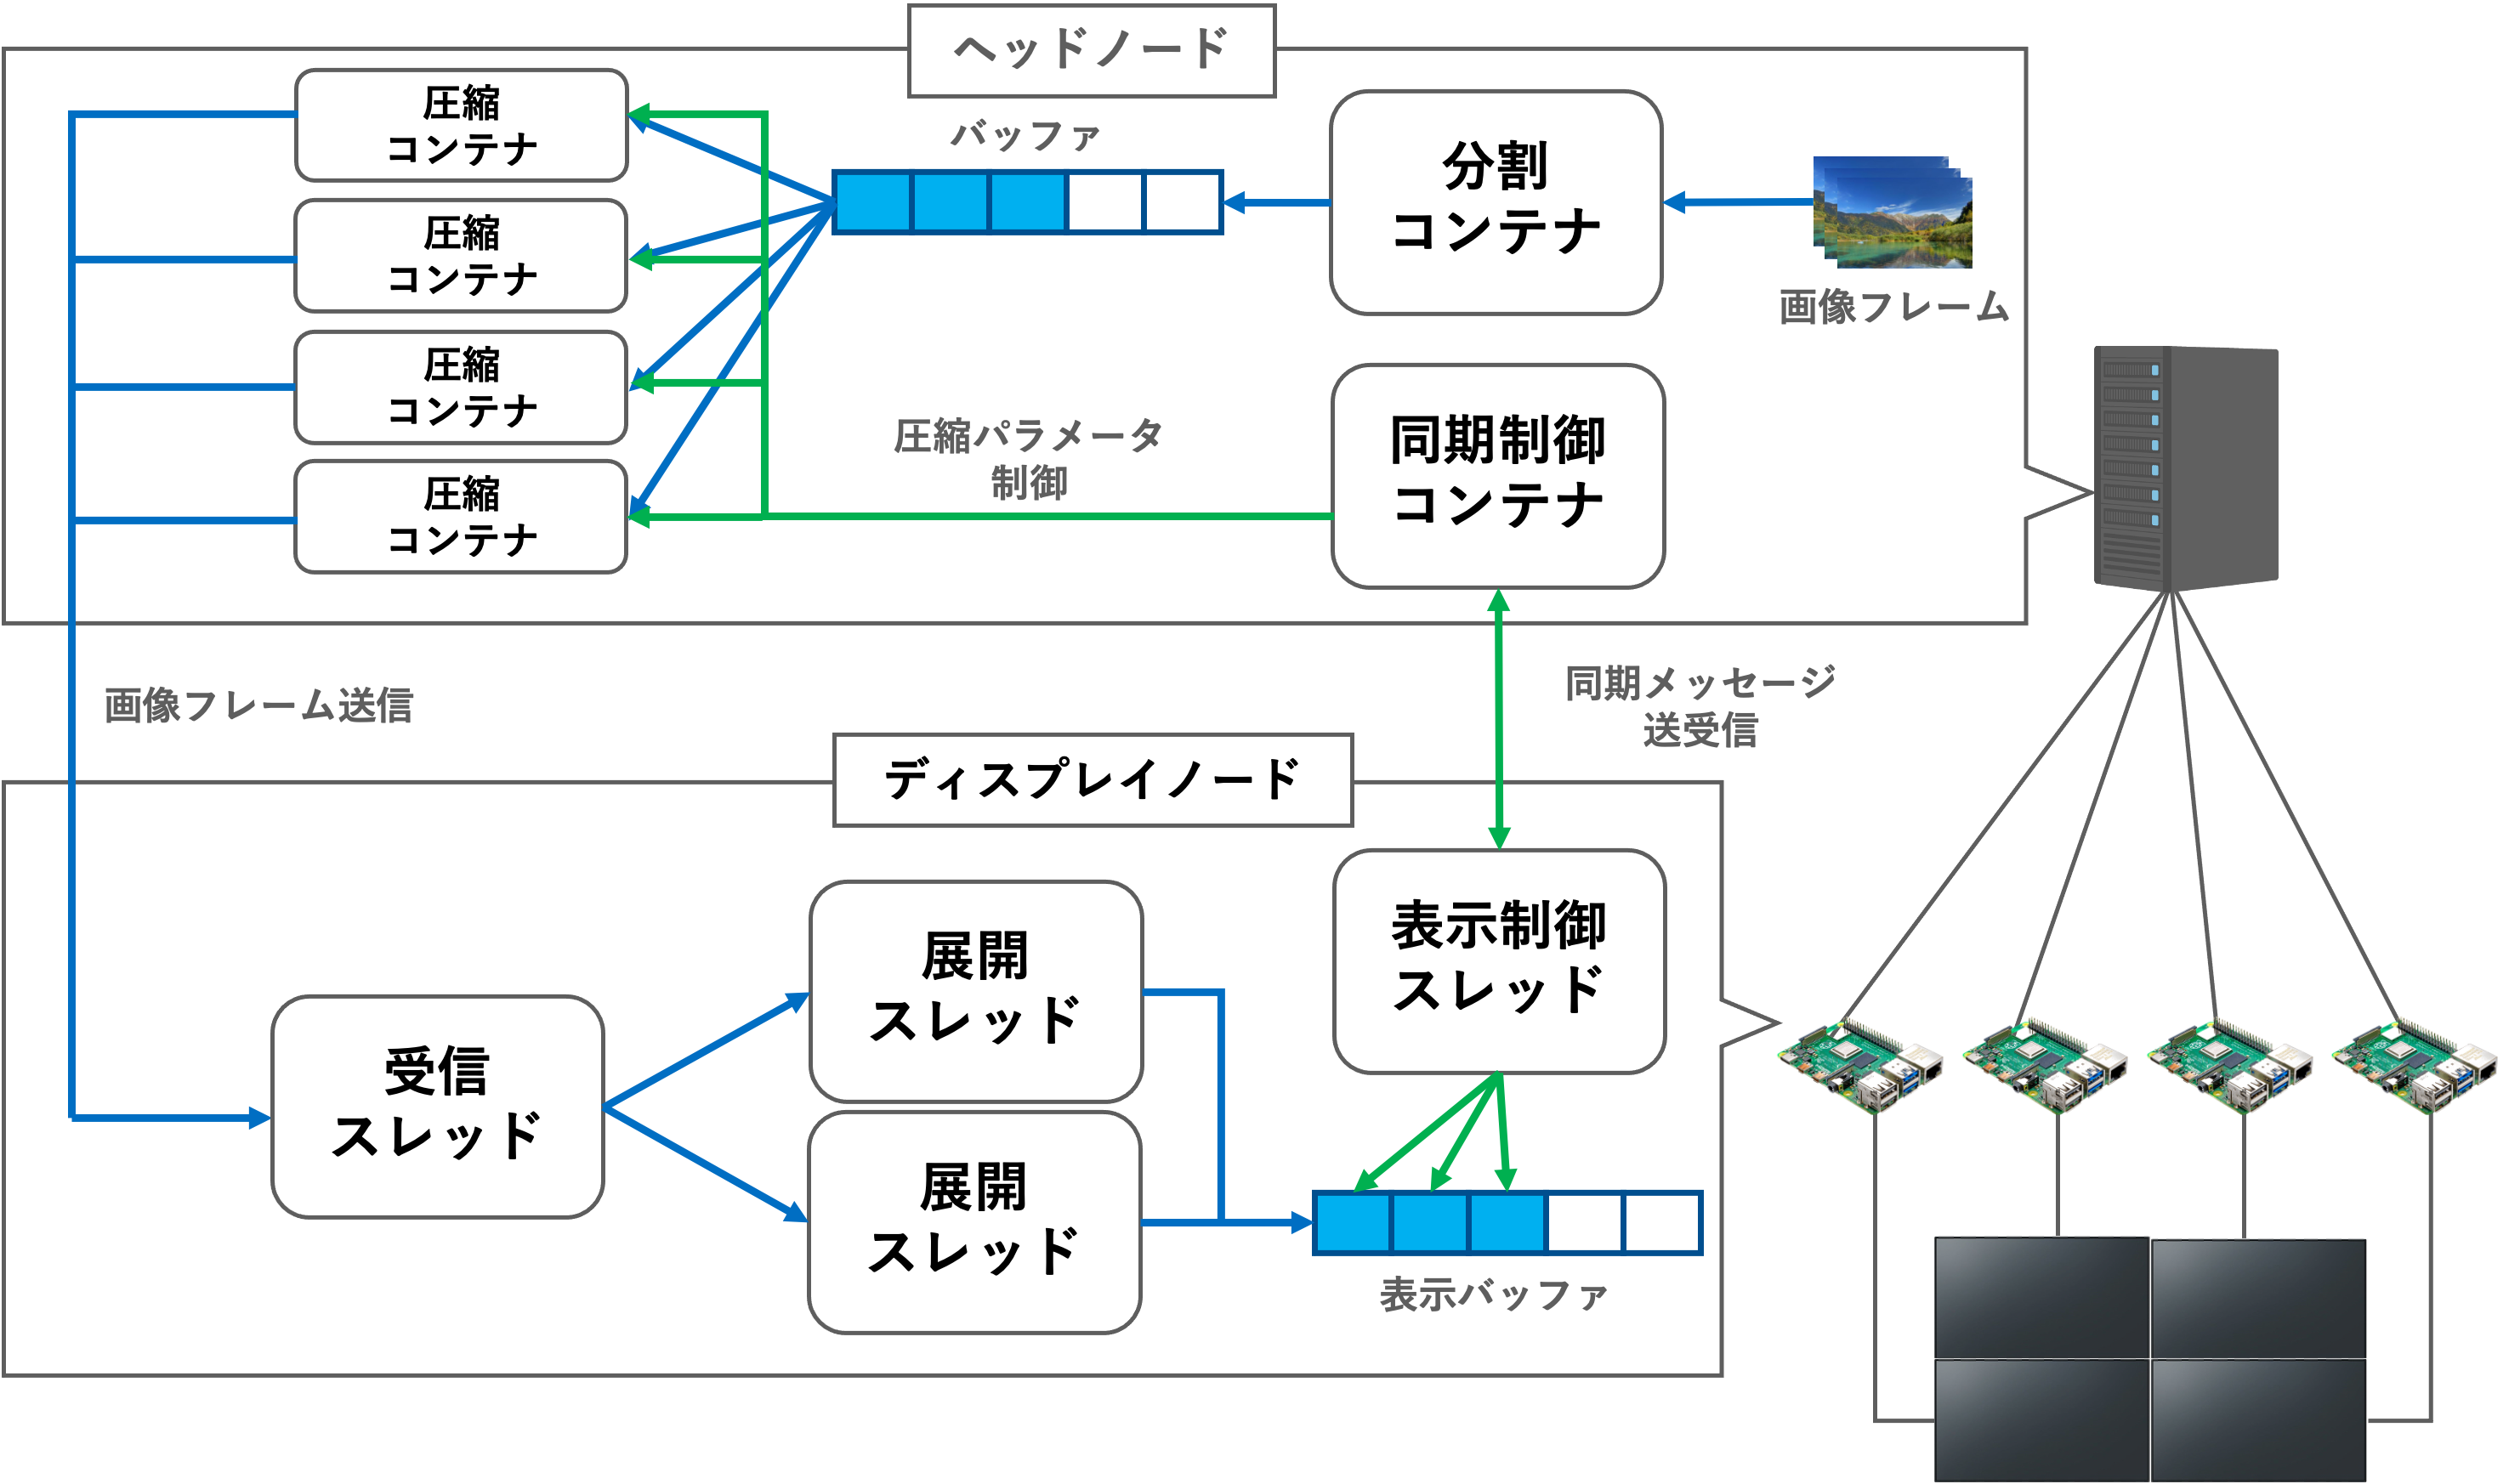
\includegraphics[width=\linewidth]{./fig/system_flow.eps}
    \hspace*{\fill}
    \caption{提案手法を用いたMDの動作フロー}
   \end{figure}
